\chapter{System Design and Implementation} \label{ch:problem-solution}

This chapter presents Pista's system design and implementation based on the current codebase. The goal is to deliver consistent, accessible, and scalable startup pitch evaluations with a clear mapping between documented claims and implemented features.

\section{Solution Approach} \label{sec:solution-approach}

The solution addresses three recurring limitations in startup evaluation: inconsistency, limited accessibility, and scalability constraints. Standardized AI criteria reduce subjective variance, a web interface broadens access, and automated processing scales without fatigue effects. Pista leverages GPT\,4 to produce structured, repeatable assessments across four dimensions with actionable feedback that is useful for founders and comparable for research.

\section{System Design} \label{sec:system-design}

\subsection{Architecture Overview}\label{subsec:architecture-overview}
Pista is implemented as a three tier web application. The presentation layer uses Next.js 15 with React (App Router). The application layer exposes API routes for evaluation, transcription, and Q\&A generation, and integrates authentication. The data layer uses Convex for real time storage, reactive queries, and server functions. Clerk provides authentication and organization contexts.

The overall workflow from user interaction to output generation is shown in Figure~\ref{fig:user-flow}.

\begin{figure}[H]
  \centering
  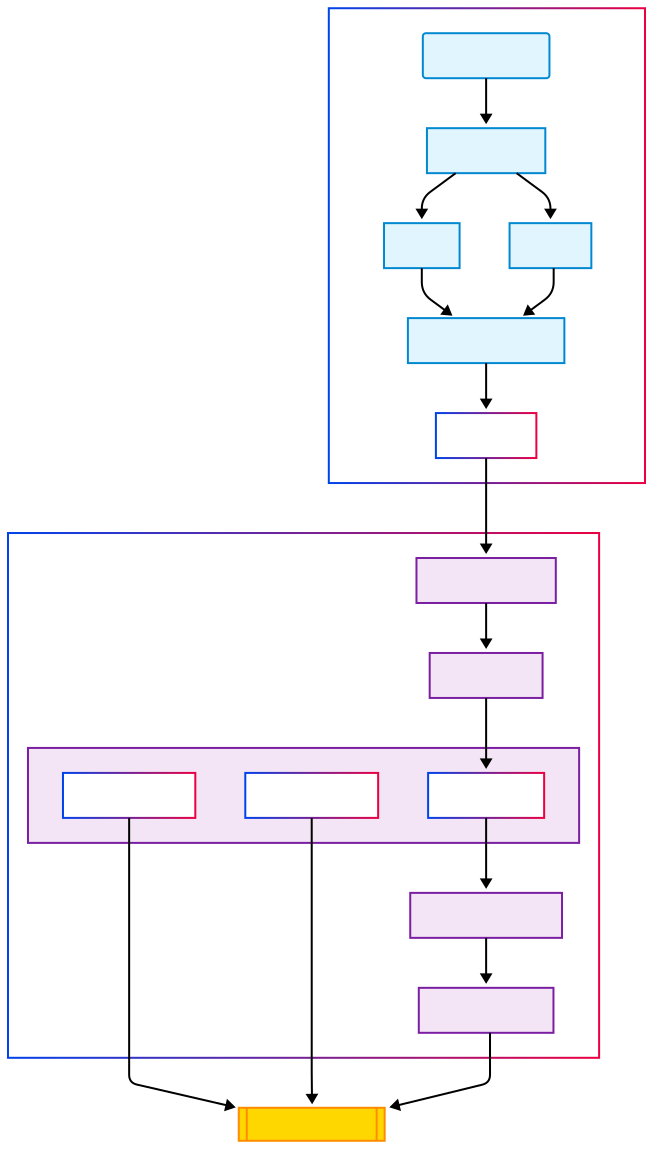
\includegraphics[width=0.85\textwidth]{img/user-diagram-flow}
  \caption{High level workflow showing user interaction and data processing}
  \label{fig:user-flow}
\end{figure}

\subsection{Evaluation Framework}\label{subsec:evaluation-framework}
The evaluation framework combines standardized criteria with prompt engineering for consistent results. Four dimensions are used with fixed weights that match the implementation:

\begin{itemize}
  \item \textbf{Problem Solution Fit} (0.30)
  \item \textbf{Business Model \& Market} (0.30)
  \item \textbf{Team \& Execution} (0.25)
  \item \textbf{Pitch Quality} (0.15)
\end{itemize}

Each dimension evaluates five aspects and yields a numeric score plus strengths and improvements. The criteria mirrors the code used in \texttt{src/app/api/evaluate/route.ts}:

\begin{lstlisting}[language=TypeScript, caption={Core evaluation criteria (excerpt)}]
const EVALUATION_CRITERIA = {
  problemSolution: {
    name: "Problem-Solution Fit",
    aspects: [
      "Problem Definition Clarity",
      "Solution Innovation",
      "Market Understanding",
      "Competitive Advantage",
      "Value Proposition",
    ],
  },
  businessModel: {
    name: "Business Model & Market",
    aspects: [
      "Revenue Model",
      "Market Size & Growth",
      "Go-to-Market Strategy",
      "Customer Acquisition",
      "Scalability Potential",
    ],
  },
  team: {
    name: "Team & Execution",
    aspects: [
      "Team Capability",
      "Domain Expertise",
      "Track Record",
      "Resource Management",
      "Implementation Plan",
    ],
  },
  presentation: {
    name: "Pitch Quality",
    aspects: [
      "Clarity & Structure",
      "Data & Evidence",
      "Story & Engagement",
      "Q&A Performance",
      "Overall Persuasiveness",
    ],
  },
} as const
\end{lstlisting}

The four dimensional processing flow is illustrated in Figure~\ref{fig:eval-flow}. This diagram matches the implemented single provider evaluation pipeline.

\begin{figure}[H]
  \centering
  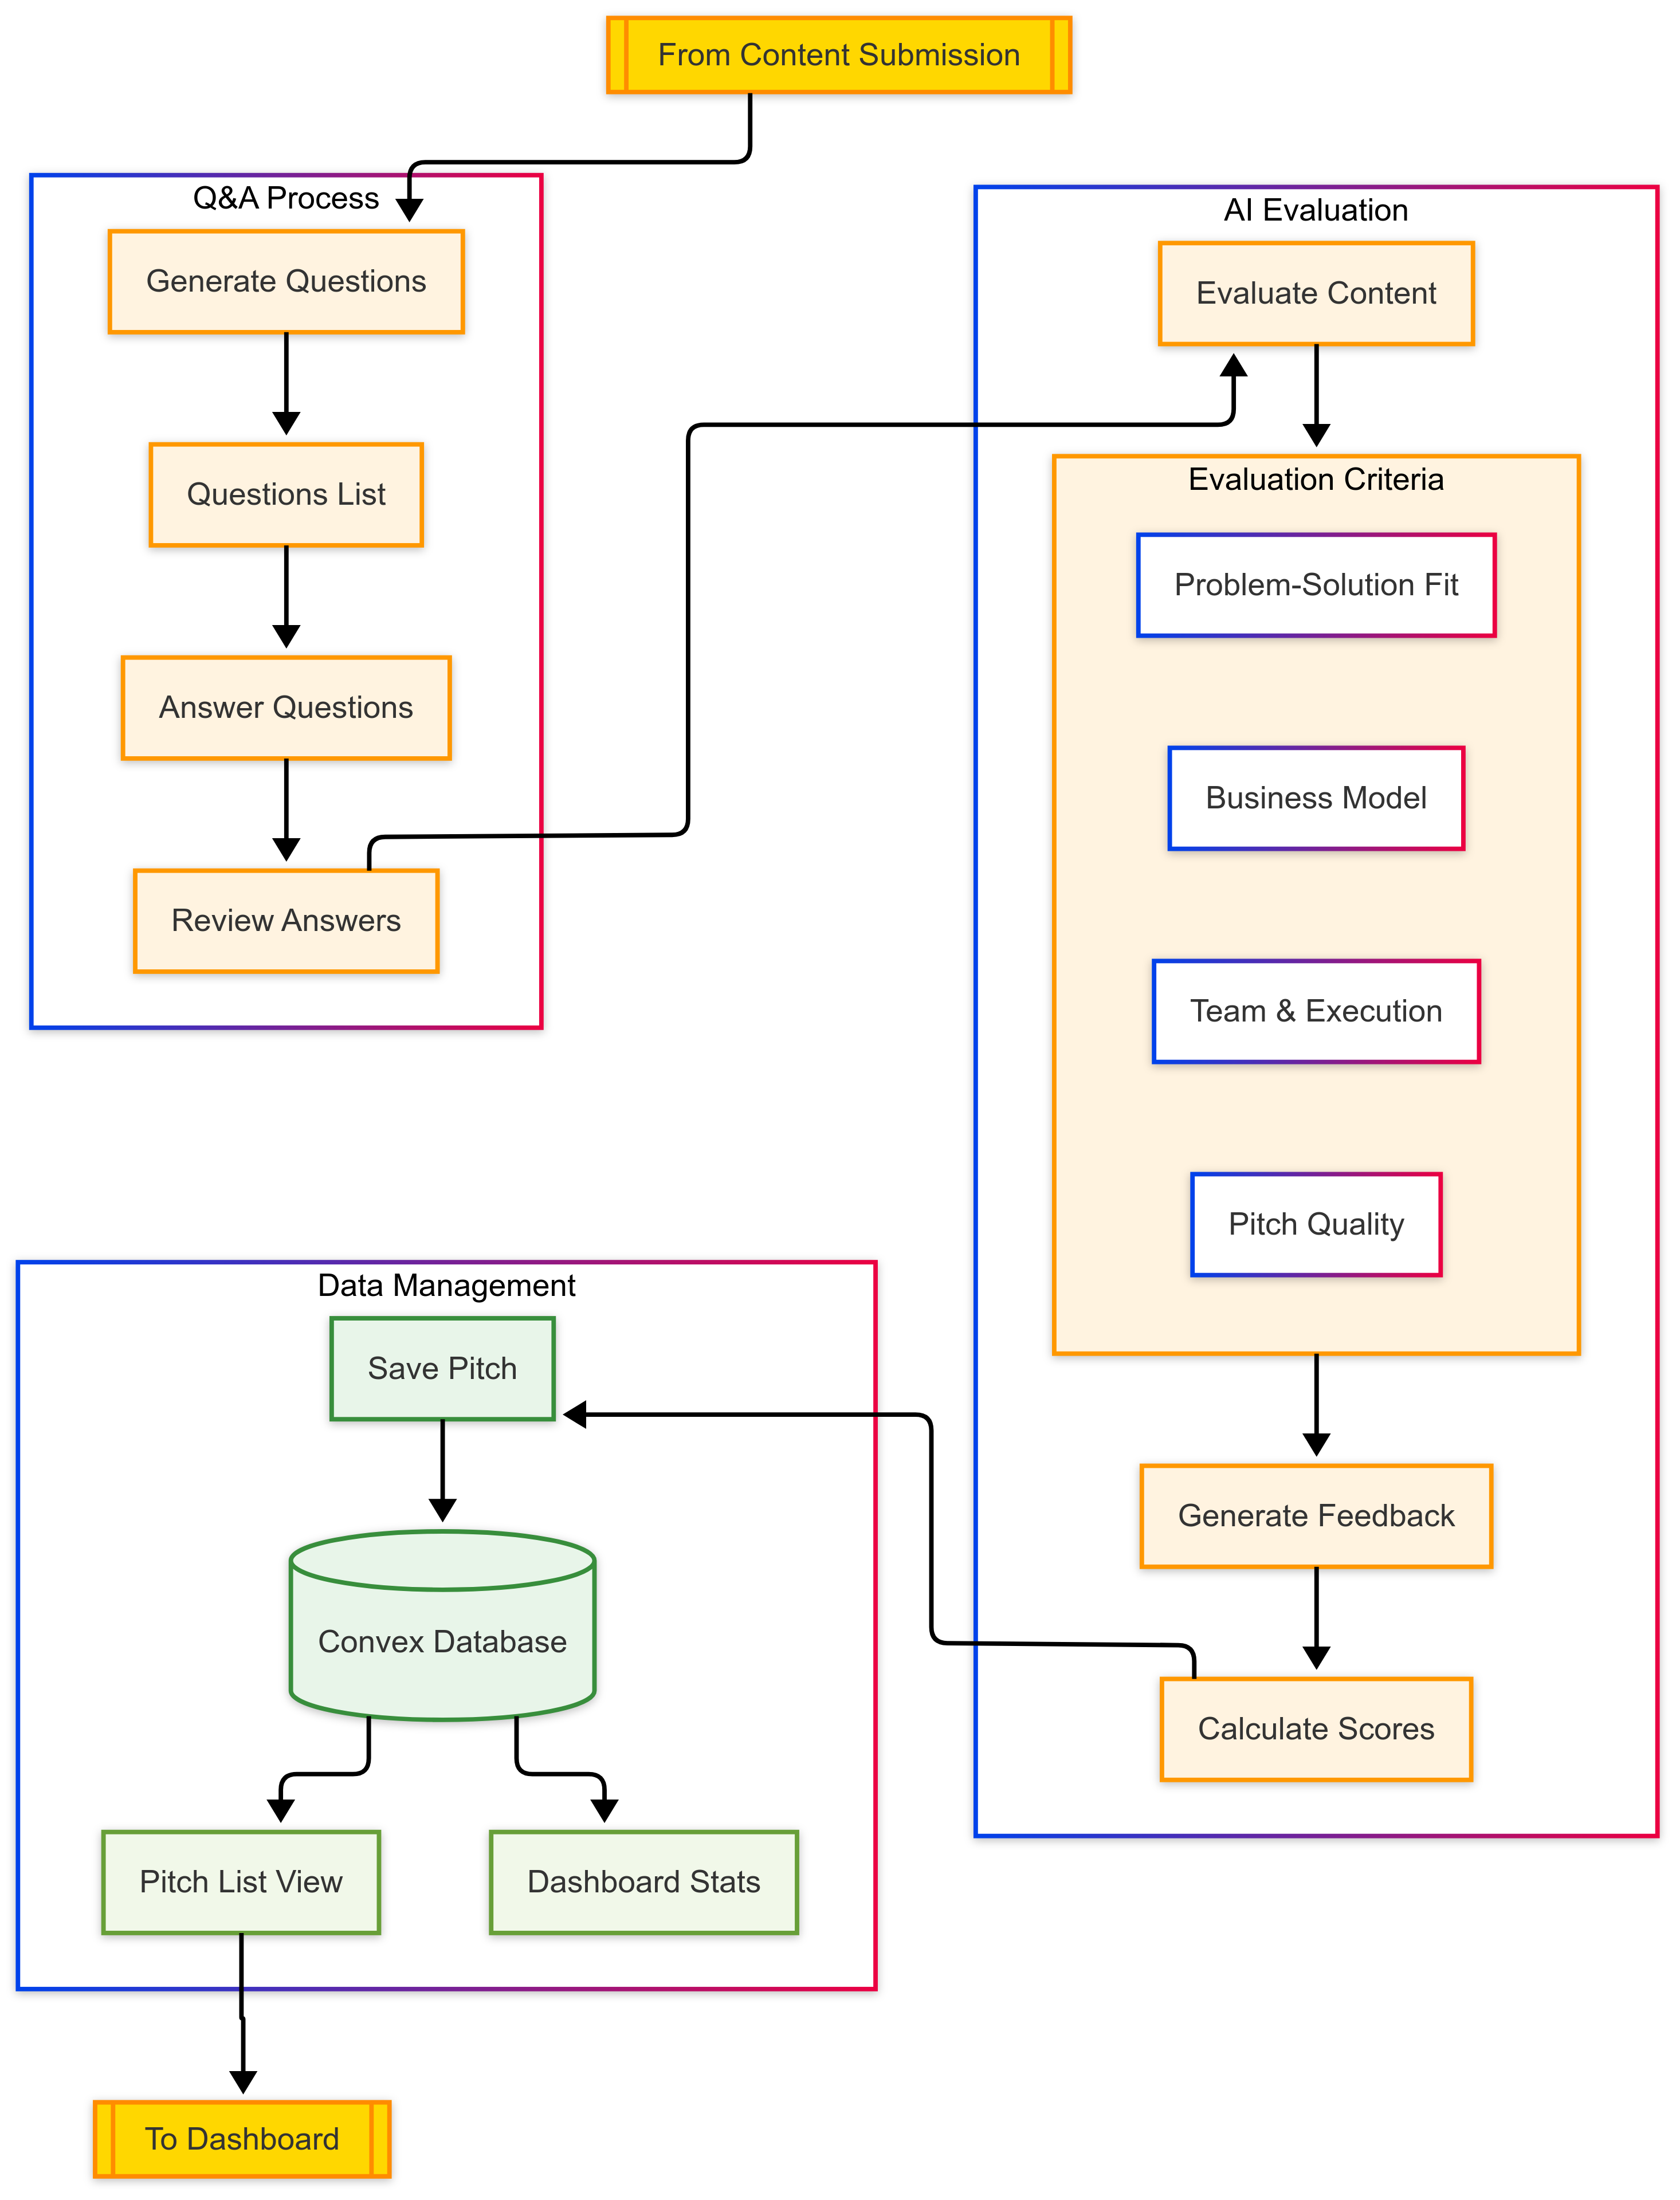
\includegraphics[width=0.9\textwidth]{img/eval-flow}
  \caption{Evaluation and processing flow across four criteria}
  \label{fig:eval-flow}
\end{figure}

\subsection{AI Integration Strategy}\label{subsec:ai-integration-strategy}
The system uses GPT\,4 through OpenAI's API. Prompts are structured to return constrained JSON for reliable parsing. Ensemble or multi provider evaluation is not part of the current implementation and is left as future work if required by the study design.

\paragraph{Prompt calibration} Initial evaluations showed central tendency with clustering near 7/10. To improve dispersion and validity, the scoring prompt was calibrated with: rubric anchors for the 1--10 scale, evidence gating that caps aspects at 4 when specifics are missing, aspect first scoring with the criterion score as the rounded average, and a reduced sampling temperature for scoring. The current configuration is tracked as \texttt{PROMPT\_VERSION = criteria\textrm{-}v1.2} and recorded in evaluation metadata.

\paragraph{Error handling} OpenAI calls use retries with exponential backoff for rate limits and transient failures. Responses are validated and mapped into strict application schemas before persistence.

\subsection{Data Models and Storage Architecture}\label{subsec:data-models-and-storage-architecture}
Convex stores pitches and user favorites with schema validation and indexed access. Each document is scoped by user and organization. Queries update the UI reactively without polling.

\paragraph{Schema overview} The \texttt{pitches} table stores title, normalized text, type, status, structured evaluation results, Q\&A pairs, organization id, user id, author name, and timestamps. Indexes include \texttt{by\_org}, \texttt{by\_user}, \texttt{by\_user\_org} and a \texttt{search\_title} index. The \texttt{userFavorites} table links users and pitches with composite indexes.

\subsection{API Endpoints and Server Functions}\label{subsec:api-and-server}
\textbf{Next.js API routes}
\begin{itemize}
  \item \texttt{/api/evaluate} evaluates text using GPT\,4 (Edge runtime)
  \item \texttt{/api/generate-questions} produces up to three follow up questions
  \item \texttt{/api/evaluate-answers} updates evaluation using Q\&A responses
  \item \texttt{/api/transcribe} transcribes audio with Whisper
\end{itemize}

\textbf{Convex functions} (\texttt{convex/pitches.ts})
\begin{itemize}
  \item Mutations: \texttt{create}, \texttt{update}, \texttt{remove}, \texttt{favorite}, \texttt{unfavorite}, \texttt{prefetch}
  \item Queries: \texttt{get}, \texttt{getPitch}, \texttt{getFilteredPitches}, \texttt{getPitchStats}, \texttt{exportCSV}
\end{itemize}

\paragraph{Q\&A generation design} The question generator asks for 1--3 high priority, evidence seeking questions and returns a structured JSON list tagged to an evaluation dimension. The route uses a lower sampling temperature for stability. If the model returns plain text, a numbered list fallback parser extracts up to three items. This improves evidence capture for the calibrated rubric without modifying the original pitch content.

\section{Authentication and Authorization Implementation}
Clerk handles sign in, session management, and organization contexts. Middleware protects routes and injects identity on the server. All Convex reads and writes are scoped by \texttt{userId} and \texttt{orgId}, which provides row level isolation without custom role tables.

\section{User Interface Implementation}
The frontend uses Next.js 15, React 18, and Tailwind CSS. Route groups organize the app into dashboard, pitch, and auth areas. Shared UI components live under \texttt{src/components/ui}; feature components live under \texttt{src/components/shared}. Lists support favorites, search, and filtering by score or date. The pitch view renders numeric scores and qualitative feedback with generated follow up questions.

The pitch creation flow is shown in Figure~\ref{fig:user-flow-pitch}. It covers text input and audio uploads, Q\&A generation, and Convex storage.

\begin{figure}[H]
  \centering
  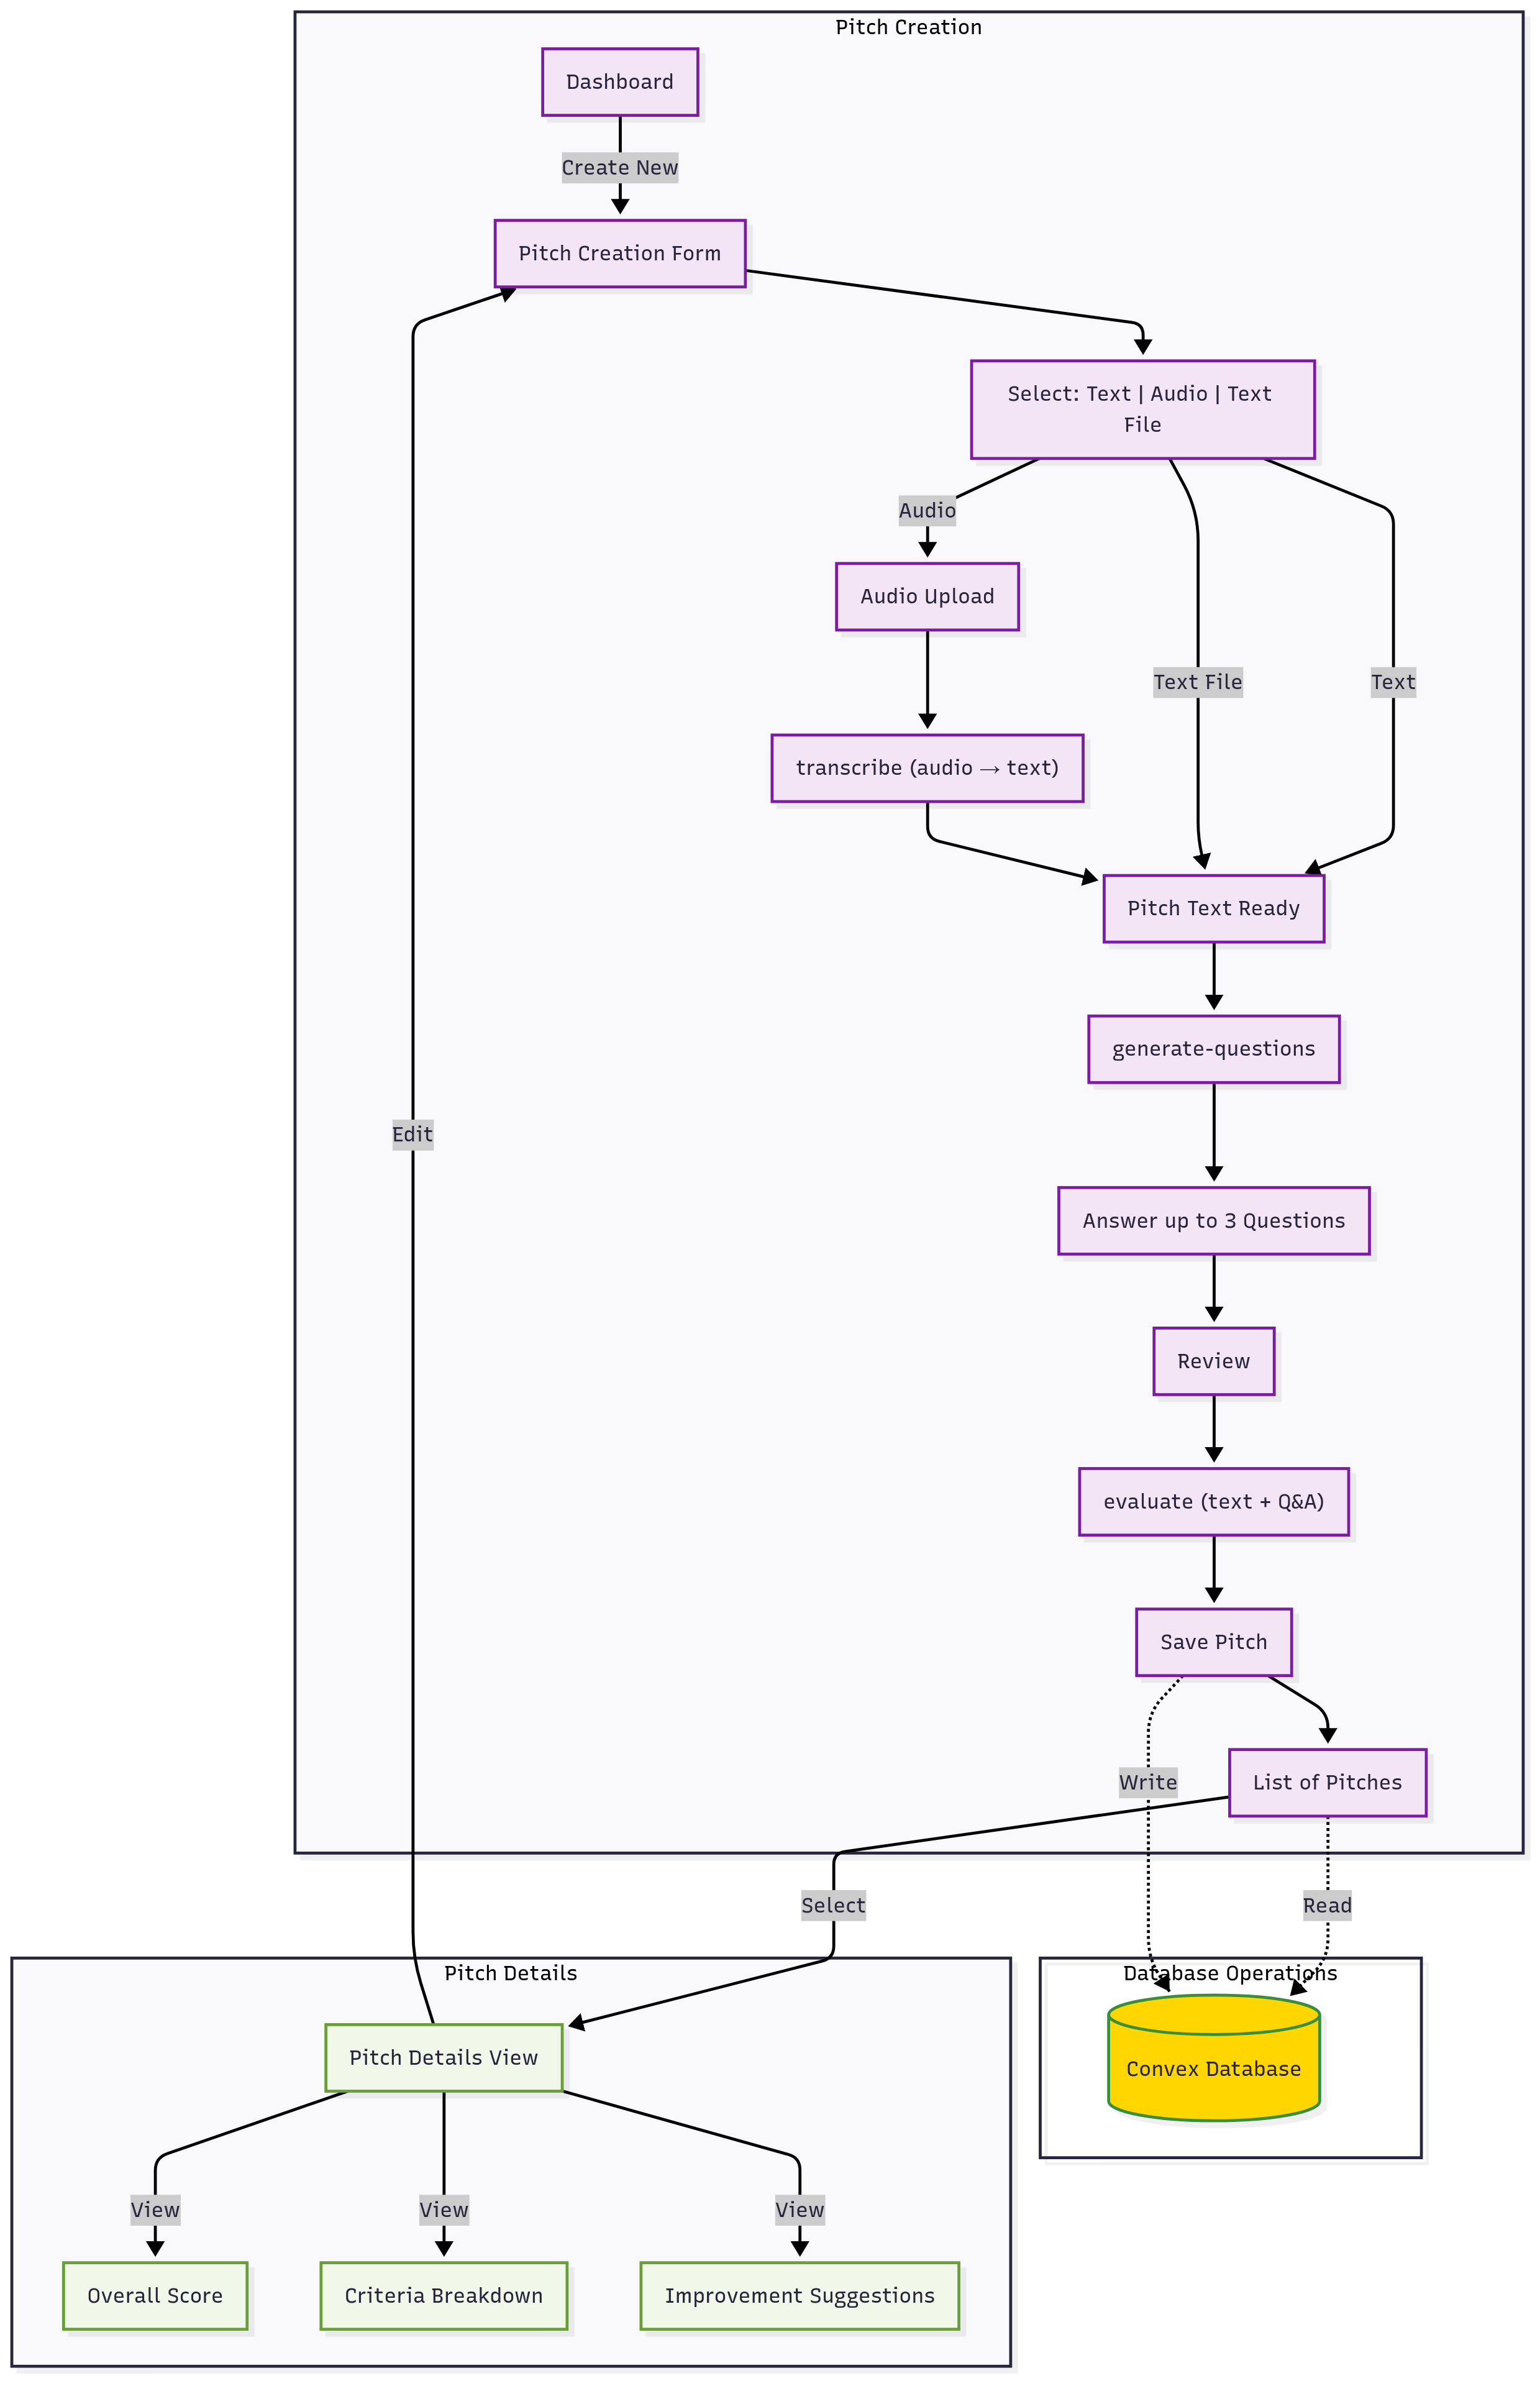
\includegraphics[width=0.9\textwidth]{img/user-flow-pitch}
  \caption{Pitch creation flow with Q\&A generation and Convex storage}
  \label{fig:user-flow-pitch}
\end{figure}

\section{Performance, Deployment, and Reliability}
\textbf{Performance} Virtualized lists maintain responsiveness with large datasets. Code splitting defers non critical UI. Reactive queries avoid manual polling.

\textbf{Deployment} API routes run on the Edge runtime where configured. Environment variables include the Convex URL, Clerk keys, and OpenAI API key. The same code paths run in development and production for result comparability.

\textbf{Reliability} API routes return clear error messages. The UI surfaces actionable feedback without exposing internal details.

\section{Implementation Results and User Experience}\label{sec:results}
Text based evaluations typically complete within 30 to 60 seconds. Audio submissions require additional time for transcription. The interface is reactive, and list updates are visible without manual refresh. These characteristics meet the design goal of responsive, consistent assessments suitable for research and iteration.
